\documentclass[class=minimal,border=10pt]{standalone}
\usepackage{tikz}
\usepackage{xcolor}
% 数学符号(\mathbb, \mathcal 等)支持
\usepackage{amsmath,amssymb}
\definecolor{base03}{RGB}{0,43,54}
\definecolor{base02}{RGB}{7,54,66}
\definecolor{cyan}{RGB}{42,161,152}
\usetikzlibrary{calc,shapes,positioning,decorations.pathreplacing,arrows.meta}
\begin{document}
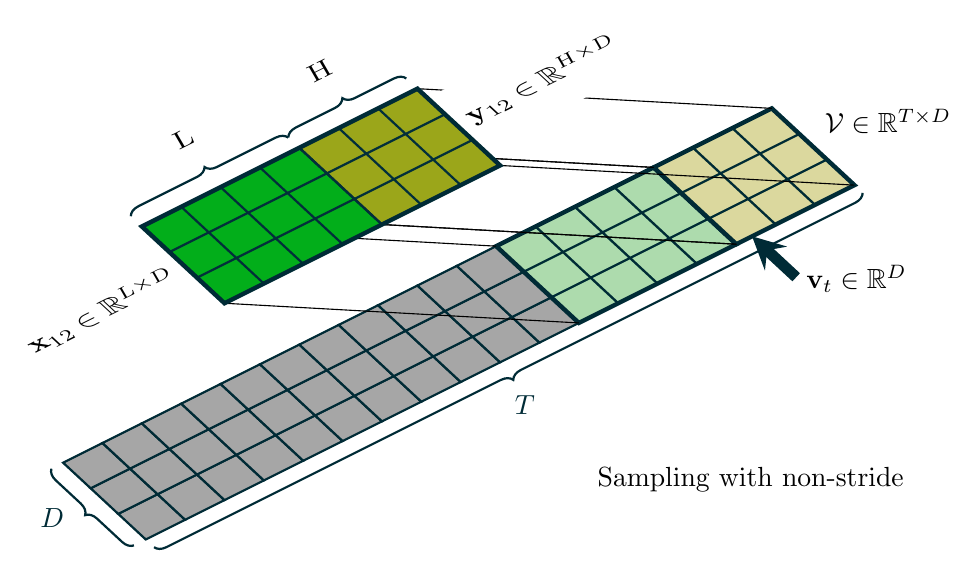
\begin{tikzpicture}[scale=.5, every node/.style={minimum size=1cm}, on grid]
    % 固定画布大小(避免不同帧因标签/布局轻微变化导致整体尺寸抖动)
    % 注意:这里使用一个略大于当前图形范围的包围盒
    \path[use as bounding box] (-3,0) rectangle (20,13);
    % 变量颜色定义(每个变量一种颜色,全局供输入/输出层使用)
    \definecolor{var0}{RGB}{38,139,210}
    \definecolor{var1}{RGB}{42,161,152}
    \definecolor{var2}{RGB}{133,153,0}
    % 立体:输入平面(1×1 方格,与卷积相同的斜视)
    \begin{scope}[node/.append style={yslant=0.5,xslant=-0.7},
                    yslant=0.5,xslant=-0.7]
        % 时间序列输入:每行一个变量,横轴为时间,1×1 方格
        \draw[draw=base03, fill=gray!70, thick] (0,0) rectangle (1,1);
    \draw[draw=base03, fill=gray!70, thick] (0,1) rectangle (1,2);
    \draw[draw=base03, fill=gray!70, thick] (0,2) rectangle (1,3);
    \draw[draw=base03, fill=gray!70, thick] (1,0) rectangle (2,1);
    \draw[draw=base03, fill=gray!70, thick] (1,1) rectangle (2,2);
    \draw[draw=base03, fill=gray!70, thick] (1,2) rectangle (2,3);
    \draw[draw=base03, fill=gray!70, thick] (2,0) rectangle (3,1);
    \draw[draw=base03, fill=gray!70, thick] (2,1) rectangle (3,2);
    \draw[draw=base03, fill=gray!70, thick] (2,2) rectangle (3,3);
    \draw[draw=base03, fill=gray!70, thick] (3,0) rectangle (4,1);
    \draw[draw=base03, fill=gray!70, thick] (3,1) rectangle (4,2);
    \draw[draw=base03, fill=gray!70, thick] (3,2) rectangle (4,3);
    \draw[draw=base03, fill=gray!70, thick] (4,0) rectangle (5,1);
    \draw[draw=base03, fill=gray!70, thick] (4,1) rectangle (5,2);
    \draw[draw=base03, fill=gray!70, thick] (4,2) rectangle (5,3);
    \draw[draw=base03, fill=gray!70, thick] (5,0) rectangle (6,1);
    \draw[draw=base03, fill=gray!70, thick] (5,1) rectangle (6,2);
    \draw[draw=base03, fill=gray!70, thick] (5,2) rectangle (6,3);
    \draw[draw=base03, fill=gray!70, thick] (6,0) rectangle (7,1);
    \draw[draw=base03, fill=gray!70, thick] (6,1) rectangle (7,2);
    \draw[draw=base03, fill=gray!70, thick] (6,2) rectangle (7,3);
    \draw[draw=base03, fill=gray!70, thick] (7,0) rectangle (8,1);
    \draw[draw=base03, fill=gray!70, thick] (7,1) rectangle (8,2);
    \draw[draw=base03, fill=gray!70, thick] (7,2) rectangle (8,3);
    \draw[draw=base03, fill=gray!70, thick] (8,0) rectangle (9,1);
    \draw[draw=base03, fill=gray!70, thick] (8,1) rectangle (9,2);
    \draw[draw=base03, fill=gray!70, thick] (8,2) rectangle (9,3);
    \draw[draw=base03, fill=gray!70, thick] (9,0) rectangle (10,1);
    \draw[draw=base03, fill=gray!70, thick] (9,1) rectangle (10,2);
    \draw[draw=base03, fill=gray!70, thick] (9,2) rectangle (10,3);
    \draw[draw=base03, fill=gray!70, thick] (10,0) rectangle (11,1);
    \draw[draw=base03, fill=gray!70, thick] (10,1) rectangle (11,2);
    \draw[draw=base03, fill=gray!70, thick] (10,2) rectangle (11,3);
    \draw[draw=base03, fill=gray!70, thick] (11,0) rectangle (12,1);
    \draw[draw=base03, fill=gray!70, thick] (11,1) rectangle (12,2);
    \draw[draw=base03, fill=gray!70, thick] (11,2) rectangle (12,3);
    \draw[draw=base03, fill=gray!70, thick] (12,0) rectangle (13,1);
    \draw[draw=base03, fill=gray!70, thick] (12,1) rectangle (13,2);
    \draw[draw=base03, fill=gray!70, thick] (12,2) rectangle (13,3);
    \draw[draw=base03, fill=gray!70, thick] (13,0) rectangle (14,1);
    \draw[draw=base03, fill=gray!70, thick] (13,1) rectangle (14,2);
    \draw[draw=base03, fill=gray!70, thick] (13,2) rectangle (14,3);
    \draw[draw=base03, fill=gray!70, thick] (14,0) rectangle (15,1);
    \draw[draw=base03, fill=gray!70, thick] (14,1) rectangle (15,2);
    \draw[draw=base03, fill=gray!70, thick] (14,2) rectangle (15,3);
    \draw[draw=base03, fill=gray!70, thick] (15,0) rectangle (16,1);
    \draw[draw=base03, fill=gray!70, thick] (15,1) rectangle (16,2);
    \draw[draw=base03, fill=gray!70, thick] (15,2) rectangle (16,3);
    \draw[draw=base03, fill=gray!70, thick] (16,0) rectangle (17,1);
    \draw[draw=base03, fill=gray!70, thick] (16,1) rectangle (17,2);
    \draw[draw=base03, fill=gray!70, thick] (16,2) rectangle (17,3);
    \draw[draw=base03, fill=gray!70, thick] (17,0) rectangle (18,1);
    \draw[draw=base03, fill=gray!70, thick] (17,1) rectangle (18,2);
    \draw[draw=base03, fill=gray!70, thick] (17,2) rectangle (18,3);
        % 输入网格线(1×1)
        \draw[step=1, base03, thin] (0,0) grid (18, 3);
        % X 窗口高亮(绿色,对应 X_i)
        \draw[base03, ultra thick, fill=green!30, fill opacity=0.6] (11, 0) rectangle (15, 3);
        \draw[step=1, base03, thick] (11, 0) grid (15, 3);
        % 保存 X 窗口四角坐标,用于与输出层连线
        \coordinate (XWBL) at (11, 0);
        \coordinate (XWBR) at (15, 0);
        \coordinate (XWTL) at (11, 3);
        \coordinate (XWTR) at (15, 3);
        % Y 窗口高亮(黄色,对应 Y_i)
        \draw[base03, ultra thick, fill=yellow!40, fill opacity=0.6] (15, 0) rectangle (18, 3);
        \draw[step=1, base03, thick] (15, 0) grid (18, 3);
        % 保存 Y 窗口四角坐标,用于与输出层连线
        \coordinate (YWBL) at (15, 0);
        \coordinate (YWBR) at (18, 0);
        \coordinate (YWTL) at (15, 3);
        \coordinate (YWTR) at (18, 3);
        % 输入层尺寸与轴标注:长为 T,宽为 D,V \in R^(T×D),以及 v_t \in R^D
        % T 方向括号(沿时间轴,位于输入平面下方),
        % 文字放在括号中点附近,并向右上方微调以对齐视觉中心
        \draw[decorate,decoration={brace,mirror,amplitude=4pt},base03,thick]
            (0,-0.3) -- node[midway, below=6pt, xshift=6pt, yshift=8pt] {$ T $} (18,-0.3);
        % D 方向括号(沿特征维度,位于输入平面左侧),
        % 文字放在括号中点附近,并向右下方微调以对齐视觉中心
        \draw[decorate,decoration={brace,amplitude=4pt},base03,thick]
            (-0.3,0) -- node[midway, left=6pt, xshift=6pt, yshift=-4pt] {$ D $} (-0.3,3);
        % 这里直接使用预先构造好的数学标签文本,避免在模板中出现未转义花括号
        \node[above right=4pt] at (17.5, 1) {$ \mathcal{V} \in \mathbb{R}^{T \times D} $};
        % 选取某一时刻的向量 v_t(D 维)
        % 用更粗的线条和明显的箭头头部强调 v_t
        \draw[>=stealth, ->, line width=4.0pt, base03]
            (15.4, -1.6) -- (15.4, 0.0);
        \node[right=4pt] at (15.200000000000001, -1.5) {$ \mathbf{v}_t \in \mathbb{R}^{D} $};
    \end{scope}
    % 立体:输出层(长方形格子,变量数不变,上下同变量同色)
    % 整体相对于下方输入层在水平方向平移 OUTPUT_XSHIFT
    \begin{scope}[xshift=2cm, yshift=6cm,
                    every node/.append style={yslant=0.5,xslant=-0.7},
                    yslant=0.5,xslant=-0.7]
        % 输入窗口到输出单元的连线(输出层用长方形,高 OUTPUT_HEIGHT)
        % X -> 输出 X 块 (绿色,宽 kernel_size)
        \draw (XWBL) -- (0.0, 0)
              (XWBR) -- (4, 0)
              (XWTL) -- (0.0, 3.0)
              (XWTR) -- (4, 3.0);
        % Y -> 输出 Y 块 (黄色,宽 kernel_size)
        \draw (YWBL) -- (4, 0)
              (YWBR) -- (7, 0)
              (YWTL) -- (4, 3.0)
              (YWTR) -- (7, 3.0);
        % 输出:两个与输入窗口同尺寸的块,X 在前/左,Y 在后/右
        \draw[draw=base03, fill=green, thick] (0.0,0) rectangle (4,3.0);
        \draw[draw=base03, fill=yellow, thick] (4,0) rectangle (7,3.0);
        \draw[xstep=1, ystep=1, base03, thick] (0,0) grid (7, 3.0);
        \draw[base03, fill=base02, fill opacity=0.4] (0, 0) rectangle (7, 3.0);
        \draw[base03, ultra thick] (0, 0) rectangle (7, 3.0);
        % 顶部 L / H 括号
        \draw[decorate,decoration={brace,amplitude=4pt},base03,thick]
            (0.0, 3.4) -- (4, 3.4);
        \node[above=4pt] at (2.0, 3.4) {$ L $};
        \draw[decorate,decoration={brace,amplitude=4pt},base03,thick]
            (4, 3.4) -- (7, 3.4);
        \node[above=4pt] at (5.5, 3.4) {$ H $};
        % 标签:每一帧标注 X_i 和 Y_i(分别在左/右侧,带白色背景防止与网格混淆)
        \node[left=4pt, yshift=-4px, fill=white, inner sep=1.5pt]  at (0.0, 1.5) {$ \mathbf{x}_{12} \in \mathbb{R}^{L\times D} $};
        \node[right=4pt, yshift=4px, fill=white, inner sep=1.5pt] at (7, 1.5) {$ \mathbf{y}_{12} \in \mathbb{R}^{H\times D} $};
    \end{scope}
    % 画布右下角的用户自定义文字
    % 使用锚点 south east,使文字的右下角贴近画布边缘
    \node[anchor=south east] at (19.5,0.5) {Sampling with non-stride};
\end{tikzpicture}
\end{document}
